\documentclass[12pt, compress, titleprogressbar]{beamer}
\usepackage{etex}
\reserveinserts{28}

\usepackage[T1]{fontenc}
\usepackage[utf8]{inputenc}
\usepackage[spanish]{babel}
\usepackage{amsmath,amsfonts,amsthm}
\usepackage{algcompatible}
\usepackage{algorithmicx}
\usepackage{longtable}
\usepackage{algorithm}
\usepackage{hyperref}
\usepackage{graphicx}
\usepackage{listings}
\usepackage{booktabs}
\usepackage{enumitem}
\usepackage{multirow}
\usepackage{pstricks}
\usepackage{fourier}
\usepackage{amssymb}
\usepackage{times}

\usepackage[font=footnotesize,labelfont=bf]{caption}

\usepackage[scale=2]{ccicons}
\usepackage{minted}

\usepackage{ragged2e}
\justifying

\mode<presentation> {
	\usetheme{m}
}

\uselanguage{spanish}
\languagepath{spanish}
\deftranslation[to=spanish]{Theorem}{Teorema}
\deftranslation[to=spanish]{Definition}{Definición}

\title[CST]{Computing Selected Topics}

\subtitle[Computing Selected Topics]{Resistencia celular y tiempo de respuesta imunológica en un modelo para la infección del VIH}

\institute[ESCOM]{Instituto Politécnico Nacional\\Escuela Superior de Cómputo}

\author{Ian Yevgeni Hernández Sánchez}

\date{Junio 22, 2015}

\hypersetup{
	colorlinks=true,
	linkcolor=black,
	filecolor=black,
	urlcolor=black,
	citecolor=black
}

\urlstyle{same}


% \headsep = 10pt
% \headheight = 20pt

% \renewcommand{\theequation}{\arabic{equation}}
% \renewcommand{\thetable}{\thechapter.\arabic{table}}

% \setlength\parindent{0pt}

% \pagestyle{fancy}
% \renewcommand{\chaptermark}[1]{%
% 	\markboth{\thechapter.\ #1}{}%
% }

% \titleformat{\chapter}{\Huge\bfseries}{\thechapter}{1em}{\vspace{1cm}}

\floatname{algorithm}{Algoritmo}
\renewcommand{\algorithmicrequire}{\textbf{Entrada:}}
\renewcommand{\algorithmicensure}{\textbf{Salida:}}

% \newtheorem{example}{Nota}[chapter]

% \renewcommand{\headrulewidth}{0pt}
% \newcommand{\horrule}[1]{\rule{\linewidth}{#1}} % Comando para crear reglas divisoras con un argumento para su altura

\begin{document}
\renewcommand{\tablename}{Tabla}
	\maketitle

	\section{Introducción}
	\begin{frame}{Introducción}
		El curso de infección del VIH se caracteriza por la existencia de dos periodos principales:
		\begin{itemize}
			\item $\cdot$ Periodo de infección
			\item $\cdot$ Periodo de latencia
		\end{itemize}

		Se considera que el paciente ha adquirido el SIDA cuando el conteo de células-T baja hasta encontrarse entre el 20\% y el 30\%
	\end{frame}

	\begin{frame}{Introducción}
		Este modelo utiliza formalismos de autómatas celulares para describir la propagación de la infección en tejido linfoide y reproduce la dinámica de tres estados observada en pacientes infectados.\\

		Podemos observar que se forman estructuras de células infectadas propagadas por el tejido, atrapando células sanas y destruyendo el tejido.
	\end{frame}

	\section{Modelo del autómata celular}
	\begin{frame}{Modelo del autómata celular}
		Se representa la estructura de los nodos linfáticos mediante un espacio cuadrado de $L$ x $L$.\\

		Cada uno de los elementos del espacio representa una célula, la cual tiene 4 estados posibles:
	\end{frame}

	\begin{frame}{Estados posibles}
		\begin{enumerate}
			\item \textbf{Células sanas:} Representan las células $CD4^{+}$ y macrófagas.
			\item \textbf{Células infectadas-A:} Son las que han sido infectadas recientemente y no han sido reconocidas por el sistema inmunológico.
			\item \textbf{Células infectadas-B:} Son células infectadas-A, las cuales después de un tiempo ha perdido la capacidad para propagar la infección.
			\item \textbf{Células muertas:} Son células que han muerto a causa de la infección.
		\end{enumerate}
	\end{frame}

	\begin{frame}{Modelo del autómata celular}
		La configuración inicial se compone en su mayoría de células sanas, con una pequeña fracción $P_{VIH}=0.05$ de células infectadas-A, distribuidas de manera aleatoria en el espacio.\\

		Las siguientes reglas se aplican en cada periodo de tiempo transcurrido:
	\end{frame}

	\begin{frame}{Reglas de transición}
		\begin{enumerate}
			\item Una célula sana se convierte en infectada-A si tiene al menos $R_a$ células vecinas infectadas-A o $R_b$ células vecinas infectadas-B. De lo contrario permanece sana.
		\end{enumerate}

		Esta regla toma en cuenta la propagación de la infección a causa del contacto entre células. En el modelo original $R_a = 1$ y $R_b = 4$.
	\end{frame}

	\begin{frame}{Reglas de transición}
		\begin{enumerate}[start=2]
			\item Una célula infectada-A propaga la infección durante $\tau$-periodos de tiempo, luego se convierte en infectada-B.
		\end{enumerate}

		El tiempo de respuesta $\tau$ es el tiempo que necesita el sistema inmunológico para desarrollar un determinado antígeno y puede variar de 1 a 8 semanas. En el modelo original $\tau = 4$ para todas las células infectadas-A.
	\end{frame}

	\begin{frame}{Reglas de transición}
		\begin{enumerate}[start=3]
			\item Una célula infectada-B muere después de un periodo de tiempo.
			\item Una célula muerta tiene una probabilidad $P_{repl}$ de ser reemplazada por una célula nueva.\\
			Dicha célula nueva tiene $P_{infec}$ probabilidades de ser infectada-A y $1 - P_{infec}$ probabilidades de ser sana.
		\end{enumerate}

		En el modelo original $P_{repl} = 0.99$ y $P_{infec} = 10^{-5}$.
	\end{frame}

	\section{Variables del modelo}
	\begin{frame}{Variables del modelo}
		\begin{block}{Resistencia celular}
			\textbf{Parámetros que involucra:}
			\begin{itemize}
				\item $\cdot$ $R_a$
				\item $\cdot$ $R_b$
			\end{itemize}
		\end{block}

		\begin{block}{Tiempo de respuesta inmunológica}
			\textbf{Parámetros que involucra:}
			\begin{itemize}
				\item $\cdot$ $\tau$
			\end{itemize}
		\end{block}
	\end{frame}

	\plain{ 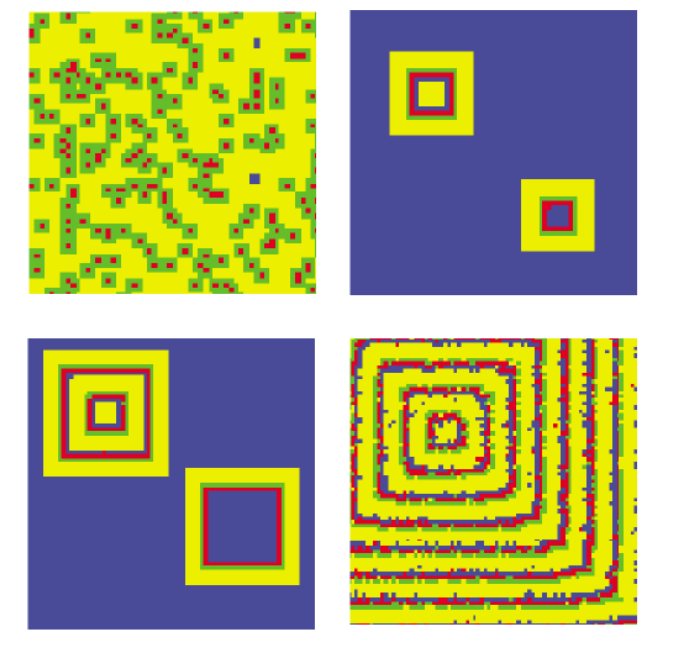
\includegraphics[height=9cm]{capturas.png} }

	\begin{frame}{Referencias}
		\begin{enumerate}
			\item Solovey G., Peruani F., Ponce S., Zorzenon R. ``On cell resistance and inmune response time lag in a model for the HIV infection''. Physica A 343 (2004). Págs. 543 - 556.\\
			\item Zorzenon R., Coutinho S. ``Dynamics of HIV infection: A cellular automata approach''. Physical Review Letters (2001), Vol. 87, No. 16.
		\end{enumerate}
	\end{frame}
\end{document}